\documentclass[11pt]{article}

\usepackage[T1]{fontenc}
\usepackage[utf8]{inputenc}
\usepackage{lmodern}
\usepackage[a4paper,margin=27mm]{geometry}
\usepackage{amsmath,amssymb,amsthm,mathtools}
\usepackage{booktabs}
\usepackage{array}
\usepackage{enumitem}
\usepackage{xcolor}
\usepackage{microtype}
\usepackage{listings}
\usepackage{tikz}
\usetikzlibrary{arrows.meta,positioning}
\usepackage[hidelinks]{hyperref}
\usepackage{url}

\definecolor{fabricblue}{HTML}{1F5B99}
\definecolor{fabricpurple}{HTML}{6D4AA2}
\definecolor{fabricorange}{HTML}{D97728}
\definecolor{codegray}{HTML}{F4F5F7}

\hypersetup{
  colorlinks=true,
  linkcolor=fabricpurple,
  citecolor=fabricblue,
  urlcolor=fabricblue,
  pdftitle={Cognitive Fabric: An Executable Formalism for Snapshot-Consistent Adaptive Coalitions of Local Experts},
  pdfauthor={Rob Tharpe}
}

\lstdefinestyle{fabric}{
  backgroundcolor=\color{codegray},
  basicstyle=\ttfamily\small,
  breaklines=true,
  frame=single,
  rulecolor=\color{black!15},
  showstringspaces=false,
  columns=fullflexible
}

\theoremstyle{definition}
\newtheorem{definition}{Definition}[section]
\newtheorem{assumption}[definition]{Assumption}
\newtheorem{remark}[definition]{Remark}
\theoremstyle{plain}
\newtheorem{theorem}[definition]{Theorem}
\newtheorem{lemma}[definition]{Lemma}
\newtheorem{corollary}[definition]{Corollary}
\newtheorem{proposition}[definition]{Proposition}

\newcommand{\R}{\mathbb{R}}
\newcommand{\N}{\mathbb{N}}
\newcommand{\clip}[3]{\left[#1\right]_{#2}^{#3}}
\newcommand{\softmax}{\operatorname{softmax}}
\newcommand{\logit}{\operatorname{logit}}
\newcommand{\arglexmin}{\operatorname{lexmin}}
\newcommand{\modelid}{\texttt{CF-1XQ-1.1}}

\title{\vspace{-8mm}
  \textbf{Cognitive Fabric: An Executable Formalism for\\
  Snapshot-Consistent Adaptive Coalitions of Local Experts}\\[2mm]
  \large 1Xq Mathematical Architecture Specification, Revision 1.1
}
\author{Rob Tharpe}
\date{July 28, 2026}

\begin{document}
\maketitle

\begin{abstract}
This paper specifies a Cognitive Fabric as a finite, immutable registry of
localized selector experts evaluated against an explicit context.  A selector
is defined as a reversible coordinate chart, a bounded positive-definite
precision geometry, and a complete family of candidate scoring models.  An
exactly optimized bounded coalition combines selector reports through a
prior-tempered logarithmic opinion pool.  A posterior-alignment certificate
separates winning confidence, agreement, independent support, redundancy,
dissent, uncertainty, and novelty.  Structural proposals are typed,
evidence-bearing advisory values and are deliberately excluded from the state
transition.

The principal results are: composition reversibility; certified lower, upper,
and condition-number bounds for selector precision; local and coalition
simplex invariants; vote-mass conservation; exact optimality of the bounded
coalition; a tempered log-pool identity and a corrected stabilized
prior-neutrality result;
deterministic replay for an explicit clock and seed; per-resolution snapshot
consistency; mechanically checked bounded-queue conservation, commit
classification, and foreign-source isolation in the abstraction; generation
monotonicity; and
structural-proposal non-interference.  The publication protocol is specified
as a TLA+ transition system.  TLAPS proves its safety invariant for arbitrary
admissible parameters: 747 obligations were proved, followed by a clean
Isabelle reconstruction run.  TLC supplies a finite-state cross-check.  A
standard-library Python implementation is presented as one finite-precision
realization, together with executable conformance tests.  Algebraic claims are
stated over exact reals; machine claims are explicitly tolerance-bounded and
rely on the stated Python lock semantics and SHA-256 collision-resistance
assumption.
\end{abstract}

\noindent\textbf{Keywords:}
mixture of experts; formal architecture; snapshot consistency; opinion pool;
coalition selection; reversible transforms; immutable generations; auditable
adaptive systems.

\section{Introduction}

Adaptive decision systems often combine routing, expert models, online
learning, uncertainty heuristics, and concurrent state publication in one
implementation.  Such a program can be useful while remaining difficult to
reason about: terms such as ``selector'', ``coalition'', and ``posterior'' may
denote whatever the current code happens to compute, and concurrency claims
may depend on accidental runtime behavior.

The Cognitive Fabric takes the opposite direction.  It first fixes a
mathematical state space and an evaluation relation.  The implementation is
then judged as a realization of that model.  A decision is not only a candidate
identifier.  It is an immutable certificate containing the source generation
and fingerprint, the explicit evaluation context, every evaluated selector
vote, the exact bounded coalition, the generalized posterior, alignment
diagnostics, and any structural advisories.

The contribution is not a claim that local experts, spline models, reversible
maps, probability pooling, or immutable versions are individually new.
Mixtures of local experts have a long history
\cite{jacobs1991,jordan1994,shazeer2017}; logarithmic pooling belongs to the
literature on combining expert distributions \cite{genest1986,hinton2002};
invertible representations are central to normalizing-flow work
\cite{dinh2016}; and versioned state is foundational in concurrency control
\cite{reed1978,lamport1994}.  The defensible contribution is their precise
composition into an auditable adaptive architecture with cross-layer
invariants, an explicit refinement boundary, and executable evidence.

\subsection{Contributions}

This specification contributes:

\begin{enumerate}[leftmargin=*,itemsep=2pt]
  \item exact definitions of a selector, selector vote, bounded coalition,
  operational posterior, posterior alignment, structural proposal, snapshot,
  decision, outcome, and publication transition;
  \item a precision construction whose spectral floor, ceiling, and condition
  bound hold by construction rather than by an approximate diagnostic;
  \item an exact coalition optimizer over the bounded evaluated set, with a
  canonical tie rule and a maximum of fifteen feasible coalitions under the
  default preselection bound;
  \item a prior-tempered logarithmic opinion pool with nonnegative prior
  residual weight;
  \item a pure evaluation relation once logical time and exploration seed are
  explicit;
  \item a TLA+ snapshot-publication protocol with a TLAPS-checked inductive
  safety theorem, plus a restricted-history implementation linearization-point
  argument and in-process exception safety for queued evidence; and
  \item a formal-to-code traceability map and an executable conformance suite.
\end{enumerate}

\subsection{Scope and non-claims}

The term \emph{posterior} in this paper means the normalized distribution
defined by the operational model.  It is a generalized posterior, not an
automatic claim of calibration or equivalence to a generative Bayesian model.
The quantity named expected information gain is an entropy-weighted heuristic,
not mutual information.  Structural proposals are not self-modification:
they are advisory records with no direct transition semantics.  Learning is
not algebraically reversible.  The proved reversibility is coordinate
reversibility; state rollback requires retention of an earlier immutable
snapshot.  Property tests are evidence of conformance, not machine-checked
proofs.  The TLA+/TLAPS result is a machine-checked theorem about the abstract
publication module; it is not yet a statement-level refinement proof for the
Python interpreter, nor a generic linearizability proof against an atomic
reference object.  It does not mechanize the selector reversibility, coalition,
posterior, or structural-proposal theorems, which remain mathematical proofs
with conformance tests.

\section{Architectural overview}

Figure~\ref{fig:architecture} shows the separation of immutable state,
evaluation, delayed evidence, and publication.

\begin{figure}[ht]
\centering
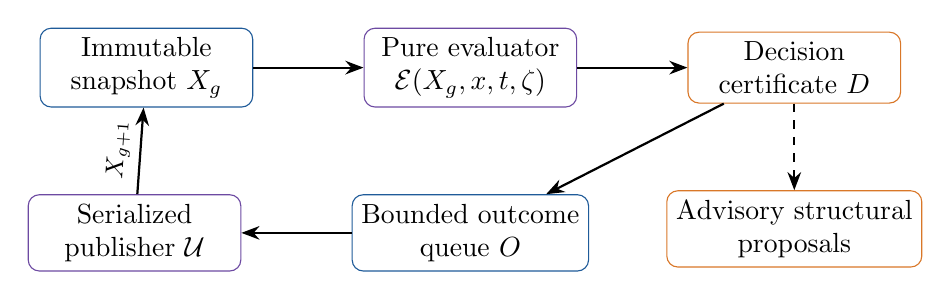
\begin{tikzpicture}[
  node distance=11mm and 14mm,
  box/.style={draw,rounded corners,minimum height=9mm,minimum width=27mm,
              align=center,fill=white},
  arrow/.style={-{Stealth[length=2.3mm]},thick}
]
  \node[box,draw=fabricblue] (snapshot) {Immutable\\snapshot $X_g$};
  \node[box,draw=fabricpurple,right=of snapshot] (eval) {Pure evaluator\\$\mathcal E(X_g,x,t,\zeta)$};
  \node[box,draw=fabricorange,right=of eval] (decision) {Decision\\certificate $D$};
  \node[box,draw=fabricblue,below=of eval] (outcomes) {Bounded outcome\\queue $O$};
  \node[box,draw=fabricpurple,left=of outcomes] (publish) {Serialized\\publisher $\mathcal U$};
  \node[box,draw=fabricorange,below=of decision] (proposal) {Advisory structural\\proposals};

  \draw[arrow] (snapshot) -- (eval);
  \draw[arrow] (eval) -- (decision);
  \draw[arrow] (decision) -- (outcomes);
  \draw[arrow] (outcomes) -- (publish);
  \draw[arrow] (publish) -- node[above,sloped,font=\small] {$X_{g+1}$} (snapshot);
  \draw[arrow,dashed] (decision) -- (proposal);
\end{tikzpicture}
\caption{The evaluator consumes one immutable generation.  Structural
proposals branch from the decision but cannot mutate the snapshot.  Only the
serialized publisher constructs and swaps a successor generation.}
\label{fig:architecture}
\end{figure}

The architecture has three boundaries:

\begin{description}[leftmargin=31mm,style=nextline]
  \item[Evaluation boundary.] A resolution captures exactly one snapshot
  reference and returns a complete decision certificate.
  \item[Evidence boundary.] Outcomes are bound to the exact source snapshot
  identity.  At publication, queued stale or foreign-branch outcomes are
  classified as rejected; before publication, bounded overflow may instead
  count them as dropped.
  \item[Publication boundary.] A valid evidence batch is folded into a new
  immutable generation and published atomically at the in-process API boundary
  under the two assumed locks.  This is neither crash atomicity nor durable
  atomicity.  The prior snapshot is not mutated.
\end{description}

\section{Preliminaries and admissible snapshots}

Let $d\in\N_{>0}$ be the common dimension.  For $a\le b$, define
\[
  \clip{x}{a}{b}=\min(b,\max(a,x)).
\]
Let $\epsilon=10^{-12}$ and
$\operatorname{saf}(x)=\clip{x}{\epsilon}{1}$.  All sets below are finite.
The implementation represents semantic registries in ascending identifier
order.

\begin{definition}[Snapshot]
An immutable Cognitive Fabric snapshot is
\[
  X=(g,\mathcal T,\mathcal C,\mathcal S,\mathcal E,\Lambda_0,\tau),
\]
where $g\in\N$ is a generation, $\mathcal T$ is a transform registry,
$\mathcal C$ a candidate registry, $\mathcal S$ a selector registry,
$\mathcal E$ a directed selector-edge registry, $\Lambda_0$ a fallback
precision model, and $\tau\in\N$ the creation time.
\end{definition}

\begin{definition}[Well-formed snapshot]
A snapshot is well formed when:
\begin{enumerate}[leftmargin=*,itemsep=1pt]
  \item transform, candidate, selector, and directed-edge keys are unique;
  \item at least one candidate is enabled and at least one selector is
  routable;
  \item every transform, selector center, precision, and spline model has
  dimension $d$, and every spline axis has a nondegenerate active domain;
  \item every transform reference and edge endpoint resolves;
  \item every selector contains exactly one model for every candidate;
  \item all semantic numbers are finite and satisfy their declared ranges;
  \item $0\le successes\le observations$, reward means lie in $[0,1]$, and
  latency means are nonnegative; and
  \item every registered transform belongs to a certified immutable transform
  variant.
\end{enumerate}
\end{definition}

The function \texttt{validate\_snapshot} enforces these conditions in the
reference realization.  Constructor inputs are canonicalized into tuples
before publication, preventing mutation of caller-owned lists from changing
an existing snapshot.

\begin{definition}[Canonical snapshot identity]
Let $\operatorname{enc}(X)$ be a type-tagged, field-complete canonical JSON
encoding in which registries are identifier-sorted and finite floating-point
values are encoded by their hexadecimal representation.  The implementation
identity is
\[
  h(X)=\operatorname{SHA256}(\modelid\parallel\operatorname{enc}(X)).
\]
In the mathematical model, $h$ is treated as an injective content identifier.
In the realization, direct foreign-evidence exclusion depends on SHA-256
collision resistance.
\end{definition}

\section{Reversible coordinate charts}

\begin{definition}[Certified transform]
A transform $\theta$ is a tuple
\[
  \theta=(id_\theta,F_\theta,G_\theta,\kappa_\theta)
\]
where $F_\theta:\R^d\to\R^d$ is forward evaluation,
$G_\theta:\R^d\to\R^d$ is its inverse, and
$\kappa_\theta\in\R_{\ge0}$ is a complexity cost.  Exact admissibility requires
\[
  G_\theta\circ F_\theta=I,\qquad F_\theta\circ G_\theta=I.
\]
\end{definition}

The realization provides two variants.  An orthogonal transform uses
$F(x)=Qx$ and $G(y)=Q^\top y$, with construction-time certification
$Q^\top Q\approx I$.  An affine transform uses $F(x)=Ax+b$ and
$G(y)=A^{-1}(y-b)$, with finite values, invertibility, and an induced
infinity-norm condition bound.

\begin{definition}[Transform chain]
For an ordered chain $\boldsymbol\theta=(\theta_1,\ldots,\theta_k)$, define
\[
  F_{\boldsymbol\theta}
  =F_{\theta_k}\circ\cdots\circ F_{\theta_1},
  \qquad
  G_{\boldsymbol\theta}
  =G_{\theta_1}\circ\cdots\circ G_{\theta_k}.
\]
The chain cost is $\sum_i\kappa_{\theta_i}$.
\end{definition}

\begin{theorem}[Composition reversibility]
\label{thm:reversibility}
If every transform in $\boldsymbol\theta$ is exactly admissible, then
$F_{\boldsymbol\theta}$ is bijective and
$G_{\boldsymbol\theta}=F_{\boldsymbol\theta}^{-1}$.
\end{theorem}

\begin{proof}
Successive cancellation gives
\[
 G_{\theta_1}\cdots G_{\theta_k}
 F_{\theta_k}\cdots F_{\theta_1}=I.
\]
The reverse product similarly equals $I$.  Hence the two compositions are
mutual inverses.
\end{proof}

\begin{remark}[Finite precision]
The realization does not claim bit-exact machine inversion.  Every transform
step records its reconstructed input and Euclidean backward error, and the
complete chain applies inverse transforms in reverse order and records
\[
 \varepsilon_{\mathrm{chain}}
 =\lVert G_{\boldsymbol\theta}(F_{\boldsymbol\theta}(x))-x\rVert_2.
\]
The executable contract checks this error relative to $1+\lVert x\rVert_2$.
\end{remark}

\section{Selector geometry}

\begin{definition}[Selector]
A selector is a localized transformed expert
\[
s=(id_s,\boldsymbol\theta_s,\mu_s,\Theta_s,\mathcal M_s,
   r_s,\nu_s,e_s^0,a_s^0,\ell_s^0,h_s,\mathrm{enabled}_s).
\]
Here $\boldsymbol\theta_s$ is a reversible chart, $\mu_s\in\R^d$ a center,
$\Theta_s$ a precision parameter, $\mathcal M_s$ one candidate model per
candidate, $r_s\in[0,1]$ reliability, $\nu_s\in[0,1]$ novelty tolerance,
$e_s^0\in[0,1]$ exploration floor, $a_s^0\in(0,1]$ routing floor,
$\ell_s^0\in[a_s^0,1]$ learning floor, and $h_s$ lifecycle state.
\end{definition}

A selector is not the final selection function.  It produces a structured
vote over candidates.

\subsection{Certified precision}

Let $R$ be the stored raw lower-triangular parameter and $\gamma>0$ its factor
scale.  Define
\[
L_{ij}=
\begin{cases}
0,&j>i,\\
\sqrt{\gamma}\bigl(\operatorname{softplus}(R_{ii})+10^{-6}\bigr),&j=i,\\
\sqrt{\gamma}R_{ij},&j<i.
\end{cases}
\]
Let declared bounds satisfy
$0<\lambda_{\min}<\lambda_{\max}$ and
$\kappa_{\max}\ge1$.  Set
\[
 f=\max\left(\lambda_{\min},
       \frac{\lambda_{\max}}{\kappa_{\max}}\right),\qquad A=LL^\top.
\]
For a real symmetric matrix, define the absolute row-sum bound
\[
 B(A)=\max_i\sum_j |A_{ij}|.
\]
Let
\[
\widehat A=
\begin{cases}
A,&B(A)\le \lambda_{\max}-f,\\[1mm]
\dfrac{\lambda_{\max}-f}{B(A)}A,&\text{otherwise}.
\end{cases}
\qquad
\Lambda=\widehat A+fI.
\]

\begin{theorem}[Precision spectrum and condition bound]
\label{thm:precision}
For every well-formed precision model,
\[
 fI\preceq\Lambda\preceq\lambda_{\max}I,
 \qquad
 \kappa_2(\Lambda)\le\kappa_{\max}.
\]
\end{theorem}

\begin{proof}
$A=LL^\top\succeq0$.  Since $A$ is symmetric,
$\lambda_{\max}(A)\le B(A)$.  Construction therefore gives
$0\preceq\widehat A\preceq(\lambda_{\max}-f)I$.  Adding $fI$ bounds every
eigenvalue of $\Lambda$ in $[f,\lambda_{\max}]$.  Finally,
\[
\kappa_2(\Lambda)
\le\frac{\lambda_{\max}}{f}
\le\kappa_{\max}.
\]
\end{proof}

\begin{remark}[Overflow-safe realization]
The exact theorem permits arbitrarily large finite entries of $R$ and
$\gamma$.  The realization does not first form a potentially overflowing
$LL^\top$.  It writes $L=\sqrt{\gamma}\,mN$, where
$m=\max_{ij}|(L/\sqrt{\gamma})_{ij}|$ and $\max_{ij}|N_{ij}|=1$, constructs
$NN^\top$, and compares the logarithm of its scaled row-sum bound with the
available spectral budget.  When the cap is active, homogeneity gives
\[
 \widehat A=\frac{\lambda_{\max}-f}{B(NN^\top)}NN^\top
\]
without materializing $\gamma m^2$.  Thus extreme finite factors are capped
without an intermediate infinity or NaN.
\end{remark}

\begin{corollary}[Monotone broadening]
\label{cor:broadening}
For fixed raw factor and bounds, replacing $\gamma$ by
$\alpha\gamma$, $0<\alpha\le1$, cannot increase precision in Loewner order.
\end{corollary}

\begin{proof}
The realized coefficient on the fixed PSD matrix is the minimum of a
nondecreasing linear function of $\gamma$ and a fixed cap.  Reducing
$\gamma$ decreases or preserves the PSD term while leaving $fI$ unchanged.
\end{proof}

\subsection{Activation}

For input $x\in\R^d$, let
\[
z_s=F_{\boldsymbol\theta_s}(x),\qquad
\delta_s=z_s-\mu_s,\qquad
d_s^2=\delta_s^\top\Lambda_s\delta_s.
\]
The routing activation and learning locality are
\[
a_s(x)=\max\left(a_s^0,
\exp\left(\max\left(-\frac12d_s^2,\log a_s^0\right)\right)\right),
\qquad
\ell_s(x)=\max(\ell_s^0,a_s(x)).
\]
By Theorem~\ref{thm:precision}, $d_s^2\ge0$, so
$a_s,\ell_s\in(0,1]$.

The deterministic exploration score is
\[
e_s(x)=\clip{
e_s^0+\clip{inactive_s/128}{0}{0.35}+0.15\nu_s
}{0}{1}.
\]
Despite the implementation field name, this is a ranking score rather than a
Bernoulli selection probability.

\section{Selector votes}

Let $\mathcal C^+$ be the enabled candidate set.  Candidate $c$ has a positive
prior propensity $\rho_c\in(0,1)$.  For selector $s$ and candidate $c$, the
additive B-spline score is
\[
u_{sc}(z_s)=b_{sc}
+\sum_{j=1}^{d}\sum_k\beta_{scjk}B_{jk}(z_{sj}),
\qquad
\widehat p_{sc}=\sigma(u_{sc}).
\]
For a degree-$p$ axis with knot sequence
$t_0\le\cdots\le t_m$ and $N=m-p$ basis functions, define its active domain as
\[
 I=[t_p,t_N],\qquad t_p<t_N.
\]
The Cox--de Boor basis is evaluated on $I$, with the closed right endpoint
$t_N$ defined as the final basis vector.  On this declared domain the basis is
nonnegative and partitions unity:
\[
 B_{jk}(z)\ge0,\qquad \sum_k B_{jk}(z)=1
 \quad(z\in I).
\]
Outside $I$, the score remains defined, but partition of unity is not claimed.

The local score has eight positive components:
candidate prior propensity, selector activation, spline fit, smoothed
empirical success, reward quality, freshness, selector reliability, and an
uncertainty penalty.  If these are $v_{sc1},\ldots,v_{sc8}$, define
\[
L_{sc}=\sum_{j=1}^{8}\log\operatorname{saf}(v_{scj}),
\qquad
q_{sc}=\frac{\exp(L_{sc})}
{\sum_{c'\in\mathcal C^+}\exp(L_{sc'})}.
\]
$q_s$ is the selector's local operational posterior.

For $|\mathcal C^+|>1$, define normalized entropy
\[
H_s=-\frac{\sum_c q_{sc}\log q_{sc}}{\log|\mathcal C^+|},
\]
and let $H_s=0$ for one candidate.  Define
\[
u_s=\clip{\tfrac12(1-a_s)+\tfrac12H_s}{0}{1},
\]
\[
\operatorname{support}_{sc}=q_{sc}(1-u_s),\qquad
\operatorname{opposition}_{sc}=(1-q_{sc})(1-u_s),
\]
\[
\operatorname{novelty}_s=\clip{(1-a_s)\nu_s}{0}{1},
\qquad
\operatorname{IG}_s=\clip{H_s r_s}{0}{1}.
\]

\begin{definition}[Selector vote]
A selector vote is the immutable tuple containing selector identity,
transform and reconstruction traces, activation decomposition, every local
candidate decomposition, novelty, entropy-weighted information score, and the
reason the selector entered the evaluated set.
\end{definition}

\begin{theorem}[Local simplex]
\label{thm:local-simplex}
For every evaluated selector,
\[
q_{sc}\ge0,\qquad \sum_{c\in\mathcal C^+}q_{sc}=1.
\]
\end{theorem}

\begin{proof}
Stable softmax subtracts the maximum finite logit, so at least one
exponential is one and the denominator is positive.  Normalization yields the
claim.
\end{proof}

\begin{theorem}[Vote-mass conservation]
\label{thm:vote-mass}
For every selector-candidate pair,
\[
\operatorname{support}_{sc}
+\operatorname{opposition}_{sc}
+u_s=1.
\]
Moreover,
\[
\sum_c\operatorname{support}_{sc}=1-u_s.
\]
\end{theorem}

\begin{proof}
The first identity follows by factoring $1-u_s$:
\[
q_{sc}(1-u_s)+(1-q_{sc})(1-u_s)+u_s=1.
\]
The second follows from Theorem~\ref{thm:local-simplex}.
\end{proof}

\section{Bounded exact coalitions}

The evaluator first admits the three routable selectors with highest
activation, using selector ID as the tie-break.  If selectors remain, it adds
one selector maximizing
\[
 e_s+0.01J_\zeta(id_s),
\]
where $J_\zeta$ is a deterministic SHA-256-derived jitter in $[0,1]$ for
explicit seed $\zeta$.  Thus at most four selectors enter the evaluated vote
set $V$.

\begin{definition}[Feasible coalition]
For budget $M\ge1$,
\[
\mathcal F_M(V)=
\{K\subseteq V:1\le |K|\le\min(M,|V|)\}.
\]
A coalition is represented by its ascending selector-ID tuple.
\end{definition}

For $K\in\mathcal F_M(V)$, define
\[
\operatorname{coverage}(K)
=1-\prod_{s\in K}(1-a_s),
\]
\[
\operatorname{diversity}(K)=
\begin{cases}
0,&|K|=1,\\[1mm]
\dfrac{1}{\binom{|K|}{2}}
\displaystyle\sum_{\{s,t\}\subseteq K}
\dfrac12\sum_c|q_{sc}-q_{tc}|,&|K|>1,
\end{cases}
\]
\[
\operatorname{utility}(K)
=\frac1{|K|}\sum_{s\in K}
\clip{\operatorname{IG}_s+0.5a_s}{0}{1}.
\]

For an enabled directed edge internal to $K$, let
\[
w_e=\sigma(1.2\,compat_e+IG_e
-1.1\,redundancy_e-1.2\,conflict_e).
\]
Redundancy and conflict are the corresponding weighted sums divided by the
number of internal enabled directed edges, or zero if none exist.  Complexity
is the sum of transform-chain costs.

\begin{definition}[Coalition objective]
\[
\begin{split}
\mathcal J(K)={}&1.4\,coverage(K)+0.8\,diversity(K)+utility(K)\\
&-0.9\,redundancy(K)-0.8\,conflict(K)-0.03\,complexity(K).
\end{split}
\]
The selected coalition is
\[
K^\star=\arglexmin\arg\max_{K\in\mathcal F_M(V)}\mathcal J(K).
\]
\end{definition}

\begin{theorem}[Exact bounded coalition optimality]
\label{thm:coalition}
\texttt{build\_coalition} returns $K^\star$.  If several feasible coalitions
have maximum score, it returns the lexicographically smallest selector tuple.
\end{theorem}

\begin{proof}
Identifier-sorted votes establish a canonical order.  Enumeration by
\texttt{combinations} visits every nonempty subset of sizes
$1,\ldots,\min(M,|V|)$ exactly once.  Minimizing
$(-\mathcal J(K),ids(K))$ first maximizes the score and then applies the stated
tie-break.
\end{proof}

\begin{corollary}[Bounded search]
Under the default preselection bound, at most
\[
\sum_{r=1}^{4}\binom4r=15
\]
coalitions are scored.
\end{corollary}

This is exact optimality over the evaluated vote set, not over every selector
in the registry.

\begin{remark}[Combinatorial versus arithmetic exactness]
The theorem is combinatorially exact for the stated objective: every feasible
coalition is scored.  The Python realization compares IEEE-754 score values, so
rounding can merge mathematically distinct near-ties.  It is exact over those
realized scores, with the same canonical tie rule; arbitrary-precision
agreement with exact-real ordering is not claimed.
\end{remark}

\section{Coalition posterior}

Normalize enabled prior propensities:
\[
\pi_c=\frac{\rho_c}{\sum_{j\in\mathcal C^+}\rho_j}.
\]
For any finite distribution $p$ on $\mathcal C^+$, define the common
finite-precision stabilization operator
\[
 S_\epsilon(p)_c=
 \frac{\operatorname{saf}(p_c)}
 {\sum_{j\in\mathcal C^+}\operatorname{saf}(p_j)}.
\]
Let $\widetilde\pi=S_\epsilon(\pi)$ and
$\widetilde q_s=S_\epsilon(q_s)$.  Using the same normalized operator on both
sides is essential: independently clipping prior and local components without
renormalization does not preserve neutrality at the probability floor.

For $s\in K^\star$, let
\[
\omega_s=a_sr_s,\qquad
Z_\omega=\max\left(1,\sum_{s\in K^\star}\omega_s\right),
\qquad
w_s=\frac{\omega_s}{Z_\omega}.
\]
Then $w_s\ge0$ and $W=\sum_s w_s\le1$.  With
$\widetilde\pi$ and $\widetilde q_s$ as above, define
\[
G_c=\log\widetilde\pi_c+
\sum_{s\in K^\star}
w_s(\log\widetilde q_{sc}-\log\widetilde\pi_c),
\]
\[
P(c\mid x,X)=
\frac{\exp(G_c)}{\sum_{j\in\mathcal C^+}\exp(G_j)}.
\]
The winner is the lexicographically smallest candidate ID among posterior
maximizers.

\begin{theorem}[Tempered log-pool identity]
\label{thm:logpool}
\[
P(c\mid x,X)\propto
\widetilde\pi_c^{\,1-W}
\prod_{s\in K^\star}\widetilde q_{sc}^{\,w_s}.
\]
The prior has nonnegative residual weight $1-W$.
\end{theorem}

\begin{proof}
Expanding $G_c$ gives
\[
G_c=(1-W)\log\widetilde\pi_c
+\sum_sw_s\log\widetilde q_{sc}.
\]
Exponentiation and normalization yield the result.
\end{proof}

\begin{corollary}[Stabilized prior neutrality]
\label{cor:prior-neutrality}
If every selected local report equals $\pi$, then
$P=S_\epsilon(\pi)$.  If additionally
$\min_c\pi_c\ge\epsilon$, then $P=\pi$.
\end{corollary}

\begin{proof}
The equality $q_s=\pi$ implies
$S_\epsilon(q_s)=S_\epsilon(\pi)$ because the same deterministic operator is
applied to both distributions.  Every evidence difference is therefore zero,
and softmax normalizes $\log S_\epsilon(\pi)_c$ back to
$S_\epsilon(\pi)$.  When no component is floored, $S_\epsilon(\pi)=\pi$.
\end{proof}

\begin{theorem}[Coalition simplex]
\label{thm:coalition-simplex}
\[
P(c\mid x,X)\ge0,\qquad
\sum_{c\in\mathcal C^+}P(c\mid x,X)=1.
\]
\end{theorem}

\begin{proof}
The proof is identical to Theorem~\ref{thm:local-simplex}.
\end{proof}

\section{Posterior alignment}

Posterior alignment is a diagnostic certificate, not another posterior.
Let $c^\star$ be the selected candidate.  For each $s\in K^\star$, define
\[
x_s=q_{s,c^\star},\qquad
\omega_s=a_s\widetilde r_s,\qquad
\Omega=\max\left(\sum_s\omega_s,10^{-12}\right),
\]
where $\widetilde r_s$ is the reliability used in the local component.
Define weighted mean and variance
\[
\mu=\frac{\sum_s\omega_sx_s}{\Omega},
\qquad
\sigma^2=\frac{\sum_s\omega_s(x_s-\mu)^2}{\Omega}.
\]
Then
\[
\operatorname{agreement}
=\clip{\mu(1-\sqrt{\max(0,\sigma^2)})}{0}{1},
\]
\[
\operatorname{independent}
=\clip{\mu(1-\operatorname{redundancy}(K^\star))}{0}{1}.
\]
Weighted dissent, uncertainty, and novelty masses are
\[
d=\frac{\sum_s\omega_s\,opposition_{s,c^\star}}{\Omega},
\quad
u=\frac{\sum_s\omega_su_s}{\Omega},
\quad
n=\frac{\sum_s\omega_s\,novelty_s}{\Omega}.
\]

\begin{definition}[Posterior alignment]
The alignment certificate is
\[
\mathcal A=
(P(c^\star),agreement,independent,redundancy,d,u,n,A),
\]
where
\[
\begin{aligned}
A=\Bigl[
&0.35P(c^\star)+0.30agreement+0.25independent\\
&-0.15redundancy-0.15d-0.10u-0.10n
\Bigr]_{0}^{1}.
\end{aligned}
\]
\end{definition}

\begin{proposition}[Alignment range]
\label{prop:alignment}
Every component of $\mathcal A$ lies in $[0,1]$.
\end{proposition}

\begin{proof}
All local probabilities, weights, and masses lie in $[0,1]$.  Their normalized
weighted means remain in $[0,1]$.  Since $x_s\in[0,1]$, $\sigma^2\le1/4$;
the agreement expression is bounded and then clipped.  Independent support
and the final index are explicitly clipped.
\end{proof}

\section{Structural proposals}

\begin{definition}[Structural proposal]
A structural proposal is the immutable advisory tuple
\[
\mathcal P=(op,I,E,\Phi,R,\widehat g,c,\mathsf{advisory}),
\]
where:
\begin{itemize}[leftmargin=*,itemsep=1pt]
  \item $op$ belongs to the following closed operation enum:
  \begin{itemize}[leftmargin=6mm,nosep]
    \item \path{broaden_selector};
    \item \path{create_specialist_selector};
    \item \path{disconnect_redundant_selectors}; or
    \item \path{shadow_alternative_coalition};
  \end{itemize}
  \item $I$ is a nonempty canonical selector-ID tuple;
  \item $E$ is a finite numeric evidence tuple;
  \item $\Phi$ is a finite set of stated preconditions;
  \item $R$ is human-readable rationale;
  \item $\widehat g\in[0,1]$ is an estimated, not proven, gain;
  \item $c\ge0$ is a complexity estimate; and
  \item $\mathsf{advisory}=\mathsf{true}$.
\end{itemize}
\end{definition}

The fixed proposal policy emits:
\begin{enumerate}[leftmargin=*,itemsep=1pt]
  \item \texttt{broaden\_selector} when an evaluated routing activation is
  below $10^{-3}$;
  \item \texttt{create\_specialist\_selector} when weighted novelty mass
  exceeds $0.55$;
  \item \texttt{disconnect\_redundant\_selectors} when coalition redundancy
  exceeds $0.65$; and
  \item \texttt{shadow\_alternative\_coalition} when weighted dissent exceeds
  $0.55$.
\end{enumerate}

\begin{theorem}[Proposal non-interference]
\label{thm:proposal}
Evaluation and proposal emission do not alter $X$, and no structural proposal
can change the selected candidate in the decision that contains it.
\end{theorem}

\begin{proof}
The evaluator receives an immutable snapshot and constructs new frozen
records.  Proposal construction has no reference to a state-publication
primitive.  The selected candidate is computed before proposal emission and
stored in the same immutable decision.
\end{proof}

No theorem of structural improvement or structural rollback is claimed.
Those require typed application functions, checked postconditions, retained
parent snapshots, and realized-gain evaluation.

\section{Evaluation relation and deterministic replay}

\begin{definition}[Evaluation relation]
For explicit time $t\in\N$, seed $\zeta\in\mathbb Z$, and coalition budget
$M\ge1$, write
\[
X,x,t,\zeta,M\vdash D
\]
when $D$ is constructed by:
\begin{enumerate}[leftmargin=*,itemsep=1pt]
  \item validating finite input of dimension $d$;
  \item computing geometry for every routable selector;
  \item selecting the top three activations and one deterministic exploratory
  selector if available;
  \item evaluating selected votes in selector-ID order;
  \item computing the exact bounded coalition;
  \item aggregating the tempered log-pool posterior;
  \item applying canonical candidate tie-breaking;
  \item computing alignment, novelty, and proposals; and
  \item recording $(\modelid,h(X),g,t,\zeta)$ in $D$.
\end{enumerate}
\end{definition}

When evaluation time is omitted, the realization samples the monotonic clock
once and records it.  A missing seed resolves to zero.

\begin{theorem}[Functional evaluation]
\label{thm:determinism}
For fixed $(X,x,t,\zeta,M)$, the relation
$X,x,t,\zeta,M\vdash D$ has exactly one result.
\end{theorem}

\begin{proof}
All state registries and local reports are canonicalized.  Activation ties use
selector IDs; exploratory jitter is a deterministic hash of seed and selector
ID; coalition ties use ascending selector tuples; and candidate ties use
candidate IDs.  Every downstream operation is deterministic.
\end{proof}

\begin{remark}
Bit-for-bit equality across Python builds or hardware platforms additionally
depends on IEEE-754 and \texttt{libm} behavior.  The theorem concerns the
defined realization environment or exact-real model.
\end{remark}

\begin{proposition}[Registry permutation invariance]
Permuting transform, candidate, selector, edge, or selector-candidate registry
inputs without changing semantic fields yields the same canonical snapshot and
the same decision for fixed evaluation arguments.
\end{proposition}

\begin{proof}
Construction sorts non-semantic registries by their unique identifiers.
Semantic sequences, notably transform-chain and spline-axis order, are
preserved.
\end{proof}

\section{Outcomes and generation transitions}

\begin{definition}[Outcome]
An outcome is
\[
o=(g,x,c,r,b,\lambda,t_o,D,m,h),
\]
where $r\in[0,1]$ is reward, $b\in\{\mathsf{false},\mathsf{true}\}$ is success,
$\lambda\ge0$ is latency, $t_o$ observed time, $D$ the originating decision,
$m$ the model identifier, and $h$ the snapshot fingerprint.
\end{definition}

\begin{definition}[Outcome validity]
$Valid_X(o)$ holds exactly when:
\begin{enumerate}[leftmargin=*,itemsep=1pt]
  \item $o.g=X.g$, $o.m=\modelid$, and $o.h=h(X)$;
  \item the embedded decision has the same model, generation, and fingerprint;
  and
  \item the redundant input and selected-candidate fields equal those in the
  embedded decision.
\end{enumerate}
\end{definition}

This is content binding, not cryptographic authentication.  A malicious caller
able to forge complete in-memory objects is outside the current trust model.

\begin{definition}[Pure update]
For a queue-ordered outcome sequence $O$, let $O_X$ be its valid subsequence.
The pure update is
\[
\mathcal U(X,O,t_c)=
\begin{cases}
X,&O_X=\varnothing,\\
Learn(X,O_X,t_c),&O_X\ne\varnothing.
\end{cases}
\]
For a nonempty valid batch, the successor has generation $g+1$.  Candidate
definitions, transforms, and topology are unchanged; selector models, health,
precision, and edge statistics may change.
\end{definition}

The learning fold is intentionally queue-order-sensitive.  Batch permutation
invariance is not claimed.

\begin{theorem}[Generation monotonicity and old-state preservation]
\label{thm:generation}
\[
generation(\mathcal U(X,O,t_c))-generation(X)\in\{0,1\}.
\]
The difference is one exactly when $O_X$ is nonempty.  In either case, the
original snapshot $X$ is unchanged.
\end{theorem}

\begin{proof}
An empty valid set returns the same object.  Otherwise the update constructs a
new frozen snapshot with generation $g+1$ by functional replacement.  No
operation mutates a field of $X$.
\end{proof}

\begin{theorem}[Direct foreign-evidence exclusion]
\label{thm:branch}
An outcome from a distinct same-numbered snapshot branch is not included in
the valid learning subsequence $O_X$ unless the two canonical identities
collide.  Equivalently, no such occurrence is directly applied as learning
evidence.
\end{theorem}

\begin{proof}
$Valid_X(o)$ requires both generation and fingerprint equality.  A different
canonical state has a different mathematical identity.  The implementation
conclusion is conditioned on SHA-256 collision resistance.
\end{proof}

This is an application-exclusion property, not full non-interference.  Because
the queue is bounded, a foreign outcome can occupy capacity or evict an older
local outcome before publication and thereby influence later evolution
indirectly.  Preventing that channel would require admission-time validation or
separate capacity.

\begin{proposition}[Update range safety]
For a well-formed snapshot, valid typed outcomes, and learning rates in $[0,1]$:
observation and success counts remain valid; reward means stay in $[0,1]$;
latency means remain nonnegative; selector reliability remains in $[0.01,1]$;
edge statistics remain in $[0,1]$; and updated precision satisfies
Theorem~\ref{thm:precision}.
\end{proposition}

\begin{proof}
Counts increment by nonnegative integers and success increments by zero or
one.  Running means are convex combinations.  Reliability and edge updates are
clipped.  Precision adaptation forms a convex combination in the PSD cone,
refactorizes by Cholesky, and re-enters the certified precision constructor.
\end{proof}

\section{Concurrent snapshot publication}

The reference register has two locks: a publication lock and an outcome lock.
A resolution holds the publication lock only long enough to capture one
snapshot reference.  Evaluation then proceeds outside the lock against the
captured immutable value.  Observation appends under the outcome lock.  A
publisher holds the publication lock, then the outcome lock, while it captures
the current batch, validates and learns, clears the batch only after successful
successor construction, and swaps the snapshot reference.

\begin{theorem}[Per-resolution snapshot consistency]
\label{thm:snapshot}
Every completed resolution is derived from exactly one snapshot $X$.  Its
decision satisfies
\[
D.generation=X.g,\qquad D.snapshot\_fingerprint=h(X).
\]
A concurrent publication cannot cause one decision to mix fields from two
generations.
\end{theorem}

\begin{proof}
\texttt{resolve} captures one snapshot reference under the publication lock
and passes only that reference into evaluation.  Valid snapshots are
transitively composed of canonical immutable values.  Publication constructs a
different snapshot and replaces the register reference.  It does not mutate
the captured value.  The TLAPS predicate
\texttt{ResolutionSnapshotConsistency} machine-checks the generation and
fingerprint metadata portion of this claim.  The stronger field-level
no-mixing conclusion additionally uses the Python immutable-object capture
argument and is not represented field by field in the TLA+ state.
\end{proof}

\begin{theorem}[Restricted-history implementation linearization points]
\label{thm:linearizable}
For completed in-process calls among the listed API operations, under the
stated lock semantics:
\begin{itemize}[leftmargin=*]
  \item \texttt{resolve} linearizes at its snapshot-reference capture;
  \item \texttt{observe} linearizes at its locked queue append, including any
  same-critical-section eviction and drop-count increment;
  \item an empty \texttt{publish\_generation} linearizes at the locked
  empty-queue check; and
  \item a successful nonempty \texttt{publish\_generation} linearizes at the
  snapshot-reference assignment after queue clearing and rejection accounting.
\end{itemize}
\end{theorem}

\begin{proof}
Publishers cannot overlap.  While publication holds its lock, no resolver can
capture the registry reference.  The outcome lock prevents an append from
entering the captured batch after its cut.  Thus an overlapping observation is
ordered entirely before or after publication.  From queue capture through the
snapshot assignment, the publisher holds both locks, so no public register or
counter operation can observe the intermediate clear, count update, or
reference swap.  A resolution therefore sees the complete old or complete new
snapshot.  The queue copy fixes the batch; it is not itself the successful
nonempty linearization point.
\end{proof}

\begin{theorem}[In-process rollback on successor-construction failure]
\label{thm:exception}
If successor construction raises synchronously before the commit section, then
after stack unwinding the captured outcome queue, current snapshot, and
published drop/rejection counters remain unchanged.
\end{theorem}

\begin{proof}
The queue is held under the outcome lock and is not cleared until
\texttt{apply\_outcomes} has returned a successor.  The snapshot reference is
assigned and the rejection counter updated only after that return.  Context
manager exit releases both locks.  This theorem does not cover process crash,
power loss, asynchronous interruption, durable recovery, or an arbitrary fault
after the queue-clear commit section begins.
\end{proof}

A failed publication call has no successful publication linearization point;
it stutters on the externally visible abstract state.  In the TLA+ model it may
change only publisher-local control and a ghost failure marker.

The queue has finite capacity.  When full, the oldest outcome is deliberately
discarded and \texttt{dropped\_outcomes} increments.  Stale or
fingerprint-mismatched entries are deliberately removed during a successful
publication attempt and \texttt{rejected\_outcomes} increments.  The
architecture therefore proves bounded storage and explicit accounting, not
lossless evidence retention.  The full conservation equation uses ghost sets
for queued, dropped, rejected, and applied occurrences in the TLA+ module; the
Python object exposes only drop and rejection counters.

\section{Mechanically checked publication safety}
\label{sec:mechanized}

The module \texttt{CognitiveFabricPublication.tla} makes the concurrency
boundary executable as a transition system.  Its parameter assumptions are
$R$ finite with $R\ne\varnothing$, $C\in\mathbb N_{>0}$, and
$N\in\mathbb N_{>0}$ for the resolver set, queue capacity, and bound on
distinct outcome occurrences.  Publisher control is deliberately exposed as
\[
\texttt{idle}\to\texttt{publish\_locked}\to
\texttt{building}\to\texttt{ready}\to\texttt{idle}.
\]
The action relation contains resolver capture and completion, local, foreign,
and malformed observation, the four publication phases, the empty path, and
the exception path.  The behavior specification is
\[
\mathit{SafetySpec}\ \equiv\ Init\ \land\ \Box[Next]_{\mathit{vars}}.
\]
The history function \texttt{outcomeById}, disposition sets, commit log, and
application counter are ghost state: they make occurrence identity and
accounting explicit without requiring the Python realization to store them.
In this module, a local \texttt{Observe} consumes one resolver's
\texttt{ready} token, so the direct trace correspondence assumes at most one
local observation per modeled resolution completion.  The Python API does not
enforce that client discipline and accepts repeated use of a decision.  That
difference is another explicit reason the present traceability map is not an
implementation refinement theorem.

The checked safety predicate is the conjunction
\[
\begin{split}
\mathit{Safety}\equiv{}&
\mathit{TypeOK}\land\mathit{BoundedQueue}\land
\mathit{UniqueOutcomeIds}\land\mathit{DispositionDisjoint}\\
&{}\land\mathit{OutcomeAccounting}\land\mathit{CountAccuracy}
\land\mathit{SnapshotGenerationAgreement}\\
&{}\land\mathit{PublisherLockInvariant}
\land\mathit{ResolutionSnapshotConsistency}\\
&{}\land\mathit{CorrectCommitClassification}
\land\mathit{ForeignApplicationExclusion}.
\end{split}
\]
In particular, every created occurrence belongs to exactly one of the current
queue, dropped, rejected, or applied sets; counters equal the corresponding
cardinalities; every commit partitions its cut into exactly the identifiers
valid and invalid at the captured base; and no foreign occurrence enters the
applied set.  The inductive strengthening records occurrence identity and the
source shape needed to derive direct foreign-application exclusion.

\begin{theorem}[Mechanized publication invariant]
\label{thm:tlaps-safety}
Under \texttt{ParameterAssumptions},
\[
\mathit{SafetySpec}\ \Longrightarrow\ \Box\mathit{Safety}.
\]
\end{theorem}

\begin{proof}
The accompanying proof module shows that \texttt{Init} establishes
\texttt{InductiveSafety}; proves preservation for every one of the eleven
\texttt{Next} branches; proves preservation by the stuttering branch in
$[Next]_{\mathit{vars}}$; and applies temporal induction.  TLAPS rolling
1.6.0-pre build \texttt{3ab43c7}, invoked with
\texttt{--strict --cleanfp -C}, discharged all 747 obligations.  Its final
Isabelle reconstruction reported no errors \cite{cousineau2012}.
The module also proves the failure action preserves the evidence state and that
a successful commit increments the generation exactly when its valid set is
nonempty.
\end{proof}

This is a symbolic theorem over every model instance satisfying the parameter
assumptions, rather than a finite enumeration; $N$ is nevertheless an explicit
per-instance bound on distinct occurrence identifiers.  It proves the abstract
safety predicate, not a statement-level Python refinement or a general
atomic-object
linearizability theorem.  As an independent finite cross-check, TLC
2026.03.02.213938 used $|R|=2$, $C=2$, and $N=4$.  It explored 920,549
generated states, 402,582 distinct states, and depth 38 without error, while
also checking \texttt{PublicationEventuallyReturns} under weak fairness for an
already-active publisher.  That liveness check is finite-instance evidence;
the TLAPS theorem above is a safety result.  Deadlock checking is disabled in
the TLC configuration.  The fairness condition begins only after a publisher
has acquired its lock; it asserts neither eventual client requests, lock
acquisition fairness, nor Python scheduler progress.

\section{Reference realization and traceability map}

The Python module \texttt{cognitive\_fabric\_reference.py} is one
standard-library finite-precision realization.  Table~\ref{tab:mapping} maps
formal objects to implementation symbols for auditability.  The table is a
traceability relation, not a mechanically proved refinement mapping.

\begin{table}[ht]
\centering
\small
\begin{tabular}{
  >{\raggedright\arraybackslash}p{0.36\linewidth}
  >{\raggedright\arraybackslash}p{0.56\linewidth}}
\toprule
Formal object or property & Reference symbol \\
\midrule
Certified coordinate maps &
\path{OrthogonalTransform}, \path{AffineTransform} \\
Chain inverse and backward certificate &
\path{apply_transform_chain}, \path{TransformChainTrace} \\
Certified precision &
\path{PrecisionModel.matrix}, \path{symmetric_spectral_upper_bound} \\
Selector &
\path{SelectorRegion} \\
Selector vote and $q_{sc}$ &
\path{evaluate_selector}, \path{SelectorVote},
\path{CandidateScoreDecomposition.local_posterior} \\
Coalition objective and exact optimum &
\path{score_coalition}, \path{build_coalition} \\
Tempered log pool &
\path{stabilize_distribution}, \path{aggregate_coalition} \\
Alignment certificate &
\path{posterior_alignment}, \path{PosteriorAlignment} \\
Typed advisory proposal &
\path{StructuralOperation}, \path{StructuralProposal} \\
Snapshot and well-formedness &
\path{CognitiveFabricSnapshot}, \path{validate_snapshot} \\
Canonical content identity &
\path{snapshot_fingerprint} \\
Evaluation relation &
\path{evaluate_snapshot} \\
Executable decision checks &
\path{decision_invariant_violations},
\path{assert_decision_invariants} \\
Outcome validity and pure update &
\path{outcome_matches_snapshot}, \path{apply_outcomes} \\
Concurrent register &
\path{CognitiveFabric.resolve}, \path{observe},
\path{publish_generation} \\
\bottomrule
\end{tabular}
\caption{Formal-to-code traceability map.}
\label{tab:mapping}
\end{table}

\subsection{Exact and computational assumptions}

The realization and correspondence claim is conditional on:
\begin{enumerate}[leftmargin=*,itemsep=1pt]
  \item exact-real algebra for the mathematical theorems;
  \item tolerance-bounded orthogonality and backward error for IEEE-754
  realization;
  \item finite inputs, validated constructors, overflow-safe precision
  normalization, and explicit failure rather than a returned decision when an
  unrelated arithmetic operation cannot remain finite;
  \item the lock semantics of the supported Python runtime;
  \item at most one local observation per modeled resolution completion when
  comparing Python publication traces with the TLA+ module;
  \item deterministic behavior within a fixed runtime and math library; and
  \item SHA-256 collision resistance for direct computational foreign-evidence
  exclusion.
\end{enumerate}

The Jacobi eigensolver in the code is diagnostic.  The precision theorem does
not rely on it; it relies on the certified absolute row-sum bound.

\section{Executable conformance evidence}

The accompanying \texttt{unittest} suite exercises the following conformance
properties:

\begin{itemize}[leftmargin=*,itemsep=1pt]
  \item rejection of false orthogonality and ill-conditioned affine maps;
  \item complete reverse-order chain reconstruction;
  \item mutation isolation for caller-owned matrices;
  \item certified precision floor, ceiling, and condition bounds over generated
  matrices, including an extreme finite-factor overflow regression;
  \item monotone broadening in Loewner order;
  \item B-spline nonnegativity and partition of unity on the precisely derived
  closed active domain, plus rejection of degenerate domains;
  \item canonical snapshot identity under registry permutations;
  \item rejection of duplicate, missing, unknown, and non-finite state;
  \item deterministic replay for fixed snapshot, time, seed, and input;
  \item local and coalition simplex invariants and vote-mass conservation;
  \item exact coalition agreement with independent feasible-subset
  enumeration;
  \item exact prior neutrality away from the probability floor and stabilized
  prior neutrality at the floor;
  \item consistent exclusion of disabled candidates;
  \item advisory proposal non-interference;
  \item cumulative repeated-outcome spline learning and nontrivial precision
  learning;
  \item rejection of non-Boolean outcome success values;
  \item lifecycle reachability of probation;
  \item old-snapshot preservation and generation increment;
  \item occurrence-level application of the captured queue in a two-publisher
  in-process schedule, without claiming durable exactly-once delivery;
  \item evidence retention after an injected synchronous
  successor-construction exception;
  \item explicit stale and foreign-fingerprint rejection accounting; and
  \item an in-flight resolution that completes against its captured old
  snapshot after a concurrent successor is published.
\end{itemize}

These tests are executable witnesses of conformance.  They neither substitute
for the abstract TLAPS theorem nor establish the missing Python refinement
proof.  QuickCheck established the modern property-based testing pattern
\cite{claessen2000}; Alloy and Dafny remain natural tools for
structural-state exploration and implementation verification respectively
\cite{jackson2002,leino2010}.

\section{Related work and novelty boundary}

\paragraph{Mixtures and local experts.}
Adaptive and hierarchical mixtures of local experts introduced learned gating
over specialized predictors \cite{jacobs1991,jordan1994}.  Sparse
mixture-of-experts systems scale this idea to conditional computation
\cite{shazeer2017}.  The Cognitive Fabric selector is best understood as an
interpretable, ellipsoidally gated local expert with a reversible coordinate
chart.  Its novelty is not the existence of gating.

\paragraph{Probability aggregation.}
The combination of expert probability distributions, including logarithmic
pooling, has a substantial literature \cite{genest1986}.  Products of experts
and committee machines similarly multiply or combine expert evidence
\cite{hinton2002,tresp2000}.  The contribution here is the explicit
prior-tempered identity in Theorem~\ref{thm:logpool}, its trace decomposition,
and its integration with bounded exact coalition selection.  Empirical
calibration remains to be demonstrated.

\paragraph{Coalition and ensemble selection.}
Dynamic ensemble and classifier selection choose subsets based on local
competence \cite{woods1997,caruana2004}.  Coalition-structure generation and
submodular optimization provide broader combinatorial frameworks
\cite{sandholm1999,nemhauser1978}.  Here the evaluated family is deliberately
bounded, so exhaustive enumeration gives an exact theorem rather than an
approximation claim.

\paragraph{Reversible representations.}
Normalizing flows use learned invertible transforms for tractable density
models \cite{dinh2016}.  The Cognitive Fabric does not claim to be a
normalizing flow: it contains no Jacobian likelihood objective.  Reversibility
is an architectural coordinate invariant.

\paragraph{Immutable state and concurrency.}
Versioned objects, multi-version concurrency, and read-copy-update motivate
readers operating on immutable versions while writers publish successors
\cite{reed1978,bernstein1983,mckenney1998}.  The contribution here is the
formal application to an adaptive decision registry and the binding of every
decision and outcome to canonical source state, not a new general concurrency
primitive.

\paragraph{Structural adaptation.}
Systems such as Cascade-Correlation and AdaNet learn or grow model structure
\cite{fahlman1989,cortes2017}.  This realization is intentionally weaker:
it emits typed proposals but does not apply them.  Any future claim of
self-improving structure must measure realized utility, check successor
well-formedness, and provide rollback.

\paragraph{Delayed feedback.}
Only the selected candidate receives reward feedback, placing empirical
evaluation near contextual-bandit settings \cite{li2010,chu2011}.  Regret,
calibration, and drift performance are not established by the architectural
theorems.

\section{Limitations and proof roadmap}

The present paper is strong enough to serve as a mathematical architecture
specification and arXiv systems/formalism preprint.  A competitive archival
submission should add:

\begin{enumerate}[leftmargin=*,itemsep=2pt]
  \item a statement-level refinement from the Python lock protocol to an atomic
  reference specification, with explicit call/return histories for a
  mechanically checked linearizability theorem;
  \item a mechanized algebraic development in Lean, Dafny, or a comparable
  system for precision bounds, pooling, and update range preservation;
  \item contextual-bandit and drift experiments against global predictors,
  top-$k$ mixture routers, dynamic ensemble selection, and LinUCB-style
  baselines;
  \item calibration experiments using negative log likelihood, Brier score,
  expected calibration error, and risk-coverage analysis
  \cite{guo2017};
  \item exact-search versus heuristic coalition ablations and edge-objective
  sensitivity;
  \item contention stress tests with occurrence-ID instrumentation reconciling
  created, queued, applied, dropped, and rejected outcomes; and
  \item a separate structural transaction layer with typed operation
  parameters, checked preconditions, successor validation, parent retention,
  inverse or rollback certificates, and realized-gain accounting.
\end{enumerate}

The following claims remain explicitly outside the current theorem set:
machine-exact transform inversion; cryptographic authenticity; injectivity of
SHA-256; calibrated Bayesian inference; mutual-information semantics for the
information score; batch permutation invariance; lossless bounded evidence;
global coalition optimality over the full registry; executable structural
improvement; reversible learning; crash consistency; durable exactly-once
delivery; scheduler fairness; symbolic liveness; generic full-API
linearizability; and an implementation refinement theorem.

\section{Conclusion}

The Cognitive Fabric is now specified as more than a software release.  A
selector is a validated local expert in a reversible coordinate chart.  A
coalition is the exact maximizer of a stated objective over a bounded feasible
family.  The candidate posterior is a prior-tempered logarithmic opinion pool.
Posterior alignment is an eight-part diagnostic certificate.  A structural
proposal is a typed advisory value with evidence and preconditions, not an
implicit mutation.  Evaluation is a functional relation for explicit context,
and publication constructs immutable, fingerprinted generations with
a restricted-history implementation linearization-point argument and
in-process evidence rollback.  Its publication safety core is a TLA+
transition system whose inductive invariant and temporal lifting are checked by
TLAPS, with bounded TLC evidence as a separate cross-check.

This separation makes the architecture falsifiable.  Every theorem names its
assumptions; each listed implementation object has an explicit formal
correspondence; and every non-theorem is stated as future work rather than
hidden inside a name.

\appendix

\section{Reference constants}

\begin{table}[ht]
\centering
\small
\begin{tabular}{lll}
\toprule
Quantity & Symbol & Reference value \\
\midrule
Safe probability floor & $\epsilon$ & $10^{-12}$ \\
Orthogonality tolerance & $\varepsilon_Q$ & $10^{-10}$ \\
Precision diagonal offset & $\varepsilon_L$ & $10^{-6}$ \\
Top activation admissions & $k$ & $3$ \\
Maximum evaluated selectors & $|V|$ & $4$ \\
Default coalition budget & $M$ & $4$ \\
Exploration jitter scale & & $0.01$ \\
Default outcome capacity & & $4096$ \\
Formal model identifier & & \modelid \\
\bottomrule
\end{tabular}
\end{table}

\section{Canonical decision obligations}

For a returned decision $D$, the executable checker requires:
\begin{enumerate}[leftmargin=*,itemsep=1pt]
  \item model identifier equality and nonnegative evaluation time;
  \item novelty and alignment indices in $[0,1]$;
  \item a nonempty finite coalition posterior on the simplex;
  \item canonical candidate argmax;
  \item a nonempty, duplicate-free coalition contained in the vote set;
  \item every local posterior on the simplex;
  \item chain reconstruction error within tolerance; and
  \item support plus opposition plus uncertainty equal to one for every local
  candidate record.
\end{enumerate}

\section{Reproduction commands}

\begin{lstlisting}[style=fabric]
python3 -m unittest -v test_cognitive_fabric_reference.py
python3 cognitive_fabric_reference.py

# TLAPS rolling 1.6.0-pre, build 3ab43c7
tlapm --strict --cleanfp -C \
  formal/CognitiveFabricPublicationProof.tla

# TLA Tools 2026.03.02.213938
cd formal
java -cp "$TLA2TOOLS" tlc2.TLC -workers 1 \
  -config CognitiveFabricPublication.cfg \
  CognitiveFabricPublication.tla
cd ..
\end{lstlisting}

For a separate SANY parse, set \texttt{TLAPS\_STDLIB} to the TLAPS standard
module directory and run:
\begin{lstlisting}[style=fabric]
java -DTLA-Library="$TLAPS_STDLIB" -cp "$TLA2TOOLS" \
  tla2sany.SANY formal/CognitiveFabricPublicationProof.tla
\end{lstlisting}
The recorded clean result is 747 TLAPS obligations followed by an
error-free Isabelle reconstruction.  The recorded TLC result is 920,549
generated states, 402,582 distinct states, depth 38, and no error.

\begin{thebibliography}{99}

\bibitem{jacobs1991}
R. A. Jacobs, M. I. Jordan, S. J. Nowlan, and G. E. Hinton.
\newblock Adaptive mixtures of local experts.
\newblock \emph{Neural Computation}, 3(1):79--87, 1991.
\newblock \url{https://doi.org/10.1162/neco.1991.3.1.79}.

\bibitem{jordan1994}
M. I. Jordan and R. A. Jacobs.
\newblock Hierarchical mixtures of experts and the EM algorithm.
\newblock \emph{Neural Computation}, 6(2):181--214, 1994.
\newblock \url{https://doi.org/10.1162/neco.1994.6.2.181}.

\bibitem{shazeer2017}
N. Shazeer et al.
\newblock Outrageously large neural networks: The sparsely-gated
mixture-of-experts layer.
\newblock arXiv:1701.06538, 2017.
\newblock \url{https://arxiv.org/abs/1701.06538}.

\bibitem{genest1986}
C. Genest and J. V. Zidek.
\newblock Combining probability distributions: A critique and an annotated
bibliography.
\newblock \emph{Statistical Science}, 1(1):114--135, 1986.
\newblock \url{https://doi.org/10.1214/ss/1177013825}.

\bibitem{hinton2002}
G. E. Hinton.
\newblock Training products of experts by minimizing contrastive divergence.
\newblock \emph{Neural Computation}, 14(8):1771--1800, 2002.
\newblock \url{https://doi.org/10.1162/089976602760128018}.

\bibitem{tresp2000}
V. Tresp.
\newblock A Bayesian committee machine.
\newblock \emph{Neural Computation}, 12(11):2719--2741, 2000.
\newblock \url{https://doi.org/10.1162/089976600300014908}.

\bibitem{woods1997}
K. Woods, W. P. Kegelmeyer, Jr., and K. Bowyer.
\newblock Combination of multiple classifiers using local accuracy estimates.
\newblock \emph{IEEE Transactions on Pattern Analysis and Machine
Intelligence}, 19(4):405--410, 1997.
\newblock \url{https://doi.org/10.1109/34.588027}.

\bibitem{caruana2004}
R. Caruana, A. Niculescu-Mizil, G. Crew, and A. Ksikes.
\newblock Ensemble selection from libraries of models.
\newblock In \emph{Proceedings of ICML}, 2004.
\newblock \url{https://doi.org/10.1145/1015330.1015432}.

\bibitem{sandholm1999}
T. Sandholm, K. Larson, M. Andersson, O. Shehory, and F. Tohm\'e.
\newblock Coalition structure generation with worst case guarantees.
\newblock \emph{Artificial Intelligence}, 111(1--2):209--238, 1999.
\newblock \url{https://doi.org/10.1016/S0004-3702(99)00036-3}.

\bibitem{nemhauser1978}
G. L. Nemhauser, L. A. Wolsey, and M. L. Fisher.
\newblock An analysis of approximations for maximizing submodular set
functions---I.
\newblock \emph{Mathematical Programming}, 14:265--294, 1978.
\newblock \url{https://doi.org/10.1007/BF01588971}.

\bibitem{dinh2016}
L. Dinh, J. Sohl-Dickstein, and S. Bengio.
\newblock Density estimation using Real NVP.
\newblock arXiv:1605.08803, 2016.
\newblock \url{https://arxiv.org/abs/1605.08803}.

\bibitem{reed1978}
D. P. Reed.
\newblock \emph{Naming and Synchronization in a Decentralized Computer
System}.
\newblock PhD thesis, Massachusetts Institute of Technology, 1978.
\newblock \url{https://dspace.mit.edu/handle/1721.1/16279}.

\bibitem{bernstein1983}
P. A. Bernstein and N. Goodman.
\newblock Multiversion concurrency control---theory and algorithms.
\newblock \emph{ACM Transactions on Database Systems}, 8(4):465--483, 1983.
\newblock \url{https://doi.org/10.1145/319996.319998}.

\bibitem{mckenney1998}
P. E. McKenney and J. D. Slingwine.
\newblock Read-copy update: Using execution history to solve concurrency
problems.
\newblock In \emph{Parallel and Distributed Computing and Systems}, 1998.
\newblock \url{https://www.rdrop.com/users/paulmck/RCU/rclockpdcsproof.pdf}.

\bibitem{fahlman1989}
S. E. Fahlman and C. Lebiere.
\newblock The Cascade-Correlation learning architecture.
\newblock In \emph{Advances in Neural Information Processing Systems 2},
1989.
\newblock \url{https://proceedings.neurips.cc/paper/1989/hash/69adc1e107f7f7d035d7baf04342e1ca-Abstract.html}.

\bibitem{cortes2017}
C. Cortes, X. Gonzalvo, V. Kuznetsov, M. Mohri, and S. Yang.
\newblock AdaNet: Adaptive structural learning of artificial neural networks.
\newblock In \emph{Proceedings of ICML}, PMLR 70:874--883, 2017.
\newblock \url{https://proceedings.mlr.press/v70/cortes17a.html}.

\bibitem{li2010}
L. Li, W. Chu, J. Langford, and R. E. Schapire.
\newblock A contextual-bandit approach to personalized news article
recommendation.
\newblock In \emph{Proceedings of WWW}, 2010.
\newblock \url{https://doi.org/10.1145/1772690.1772758}.

\bibitem{chu2011}
W. Chu, L. Li, L. Reyzin, and R. Schapire.
\newblock Contextual bandits with linear payoff functions.
\newblock In \emph{Proceedings of AISTATS}, PMLR 15:208--214, 2011.
\newblock \url{https://proceedings.mlr.press/v15/chu11a.html}.

\bibitem{guo2017}
C. Guo, G. Pleiss, Y. Sun, and K. Q. Weinberger.
\newblock On calibration of modern neural networks.
\newblock In \emph{Proceedings of ICML}, PMLR 70:1321--1330, 2017.
\newblock \url{https://proceedings.mlr.press/v70/guo17a.html}.

\bibitem{claessen2000}
K. Claessen and J. Hughes.
\newblock QuickCheck: A lightweight tool for random testing of Haskell
programs.
\newblock In \emph{Proceedings of ICFP}, 2000.
\newblock \url{https://doi.org/10.1145/351240.351266}.

\bibitem{lamport1994}
L. Lamport.
\newblock The temporal logic of actions.
\newblock \emph{ACM Transactions on Programming Languages and Systems},
16(3):872--923, 1994.
\newblock \url{https://doi.org/10.1145/177492.177726}.

\bibitem{cousineau2012}
D. Cousineau, D. Doligez, L. Lamport, S. Merz, D. Ricketts, and H. Vanzetto.
\newblock TLA+ proofs.
\newblock arXiv:1208.5933, 2012.
\newblock \url{https://arxiv.org/abs/1208.5933}.

\bibitem{jackson2002}
D. Jackson.
\newblock Alloy: A lightweight object modelling notation.
\newblock \emph{ACM Transactions on Software Engineering and Methodology},
11(2):256--290, 2002.
\newblock \url{https://doi.org/10.1145/505145.505149}.

\bibitem{leino2010}
K. R. M. Leino.
\newblock Dafny: An automatic program verifier for functional correctness.
\newblock In \emph{LPAR-16}, LNCS 6355:348--370, 2010.
\newblock \url{https://doi.org/10.1007/978-3-642-17511-4_20}.

\end{thebibliography}

\end{document}
